\chapter{General Introduction}

\epigraph{Natural selection cannot possibly produce any modification in any one species exclusively for the good of another species.}{--- \textup{Charles Robert Darwin}}

\minitoc[n] % minitoc without title

\section{The Evolution of Cooperation}

  \subsection{Cooperative Behaviours and their Importance in Evolutionary History}

    % Peut-être que je m'épanche un peu trop là quand même

    \subsubsection{The abundance of cooperation.} When we observe the natural world, cooperation is one of the social interactions that seems to be the most recurrent in every level of nature's complexity. In particular, its examples and pratical occurences prove to be diverse as well as much useful for numerous different species. As we will see in next Subsections, many different definitions of what really constitutes a cooperative behaviour exist. In our case, we will choose the most basic one: cooperation is a behaviour where an \emph{actor} (the individual who initiate the behaviour) will behave in such a way that is beneficial to a \emph{recipient} (the other individual with the behaviour)~\parencite{West2007a}. In particular, this behaviour may or may not be costly for the actor. Obviously, in most cooperative interactions more than two individuals are directly concerned. As such, it can sometimes even be as difficult to clearly define the actors and the recipients as extracting benefits and costs.

    As we previously stated, cooperation pervades every aspects of complexity in the living. For example, even unicellular organisms such as bacteria or microorganisms are known to frequently act in a cooperative manner. By using secreations, these organisms are capable of collective sharing and communication~\parencite{Elena2003, Keller2006, West2006}. For example, \emph{Pseudomonas aeruginoas} are known to engage in situations that are called \emph{public goods game}~\parencite{Popat2012, Harrison2013}. In particular they are capable of producing nutrients that every organisms as well as themselves can enjoy in the vicinity. However, this also means that some organisms could profit from these nutrients without having to produce anything themselves (given that producing something is costly). This is were a problem of public goods can arise: because "cheaters"~\footnote{The term "cheaters" will appear several times among the lines of this manuscript. Because this word has a particular bad connotation with regards to human actions, it may be misunderstood that we attribute a malevolent intention to the organisms. Whether, through the rest of the manuscript, It should be understood as "someone who profits from a benefit without paying any cost".} can benefit from these nutrients without contributing themselves. Interestingly, these situations are well studied in the realm of cooperative dilemma, as in economic research for example. It would also not be so far-stretched to consider that the complex network of gene interactions, where genes act together to build complex living machines may very well fall under the umbrella of cooperation. It is even more astonishing when we consider that those genes used to be independent replicators living freely~\parencite{Dawkins1976, Szathmary1995}. Finally, and in similar fashion as our previous example, multicellularity is a perfect display of high cooperation between numerous different organisms. The birth of multicellular organisms is explained by the fact that single prokaryotic organisms gathered and where incorporated as mitochondries in what are now eukaryotic cells to form complex multicellular organisms. In particular, Szathmary \& Maynard Smith even rightly considered this cooperative transition to multicellularity as one of the major transitions in evolution~\parencite{Szathmary1995}.

    \begin{figure}[hbtp]
        \begin{center}
          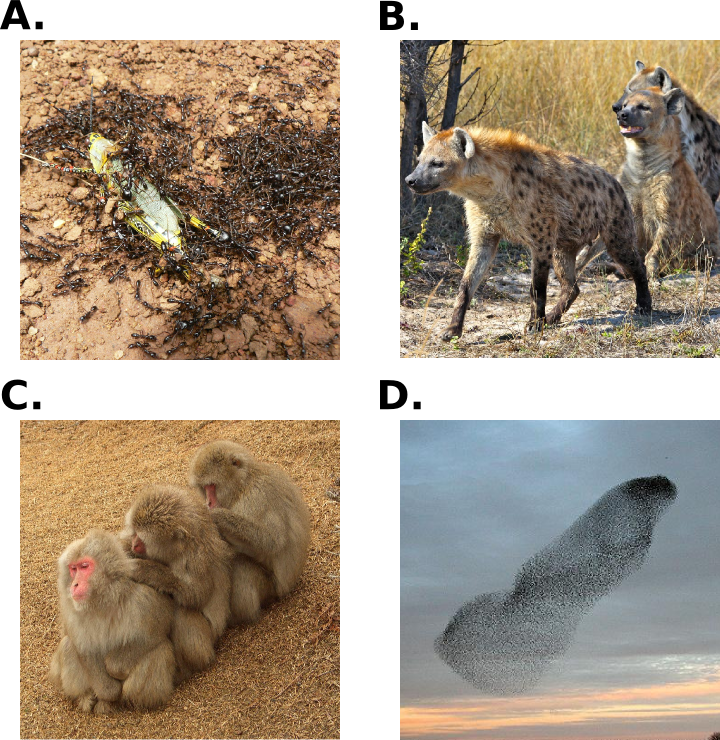
\includegraphics[scale = 0.30]{fig/Intro/CooperationExamples.png}
          \caption{\textbf{Cooperation at every level of complexity.} {\em (A)}~Eusocial insects like Hymenoptera (e.g. ants) are capable of impressive collective behaviours. {\em (B)}~Social carnivores exhibit strong cooperative behaviours and are capable of great feats of coordination during collective hunts. {\em (C)}~Social grooming is a social behaviour where individuals will groom each other reciprocally. It is thought to be a bonding exercise whose ultimate goal is to strengthen the social structure of the group. {\em (D)}~Flocs of birds are capable of the emergence of collective motions as if each individuals constituted a single bigger entity.} 
          \label{fig:CooperationExamples}
        \end{center}
    \end{figure}

    Much higher on the size scale is a popular textbook example of social behaviours: ants~(Figure~\ref{fig:CooperationExamples}~(A)). More generally, the presence of \emph{eusociality} in the animal is an astonishing display of cooperative features~\parencite{Wilson1990}. While ants are the one of the most well-known examples, insects from the Hymenoptera (i.e. ants, wasps, bees) and Isoptera (i.e. termites) orders are eusocial and represent most the insect biomass\parencite{Wilson2008}. It is interesting to note that two rodent species, the naked mole-rat and the Damaraland mole-rat, are the only vertebrates to have achieved eusociality. Eusociality might be defined as one of the highest levels of sociality and displays several impressive examples of highliy advanced cooperative actions. For example, there is cooperative care of youngs in eusocial societies, which means that individuals help raise offsprings which are not their own. Also, eusocial insects are capable of achieving efficient division of labour, which is cooperative traits where individuals specialize between several roles, eitheir to achieve several tasks simultaneously or to coordinate more efficiently. In particular, division of labour is often permanent and comes with strong morphological differences between specialized individuals. Last but not least, eusociality is also defined by a division of reproductive labor. This means that there exist reproductive and non-reproductive castes (e.g. the worker caste), which is an extreme form of cooperation between thes individuals. Because of all of these reasons, ay ants colony is often viewed as particular superorganisms wherein individuals work as one for the benefit of the group.

    If we unzoom again the lens with which we look at the world, we can find other powerful examples of cooperation among bigger vertebrates. Numerous animal species have avolved strong sociality, or presociality, which gives the opportunity to watch impressive cooperative actions in the animal world. For example, social carnivores are capable of collective hunting, where several members of the same group will be able to coordinate their actions to catch a particularly difficult or quick prey. For examples, lions are famously known for their communal and highly cooperative behaviours of collective hunting, for which they are capable of division of labour~\parencite{Scheel1991, Stander1992}. Less well-known but as much impressive, spotted hyenas~(Figure~\ref{fig:CooperationExamples}~(B)) also demonstrate high level of coordination in their collective hunting habits. While often wrongly considered but a scavenger, hyenas are also great hunters who rely on signaling and communication to coordinate~\parencite{Drea2009a, Smith2010, Smith2012a} and are capable of defending their catch against lions. The behaviours of those predators could easily be considered as complex tactics by a human observer. But even without being concerned with something as brutal as hunting, social carnivores tend to, as their name suggests, live in strongly cooperative societies. To continue with the example of spotted hyenas, they are in particular considered to be the most social among Carnivora~\parencite{Mills2003} and the complexity of their social organization is comparable to that of primates~\parencite{Drea2003}. They live in a matriarchal societies where the females dominate the males and enforce the hierarchy through agression. Non-dominant females also take care of the youngs of other females higher in the hierarchy, something which is known as alloparenting and can also be found in primates~\parencite{Small1990} and in other carnivores~\parencite{Packer2001}. Among several social species, individuals also engage in social grooming~(Figure~\ref{fig:CooperationExamples}~(C)), where they will clean each other and which is an important bounding activity which strengthen the social structure of the groop~\parencite{Spruijt1992}. Finally, we can also quickly mention the behaviours of sentinels for example in birds like the Arabian babbler~\parencite{Wright2001} or meerkats~\parencite{CluttonBrock1999}. Individuals who adopt these behaviours will act as watchers for other individuals in their group, responsible for looking for predators coming and warn the other individuals, sometimes thus taking the risk of attracting attention to themselves.

    Anyone may also have been amazed by the collective motion of flocks of birds~(Figure~\ref{fig:CooperationExamples}~(D)), as if they moved as one. Animals might sometimes organize into flocks, herds or schools from which will emerge a collective behaviour~\parencite{Couzin2002, Couzin2003}. In particular, what is impressive is that the collective cohesion achieved is due to individual behaviours and does not require a particular central decision. These social behaviours are beneficial to the individuals that constitute the groups because it can for example increase group vigilance, confuse predators, decrease the risk for each individual to be attacked or even allow to organize an active defense against a predator~\parencite{Hamilton1971, Olson2013}.

    For the moment we simply gave examples of cooperation between members of the same species (intraspecific cooperation). Yet if we unzoom again we can observe also cooperation between individuals of different species (interspecific cooperation). Often called mutualism (as we will talk about later), this form of cooperation is abundant~\parencite{Bshary2004}. For example, most plants require pollinators in order to transport their pollen so that they can succesfully pollinate the flowers. In exchange, the pollinators, whose most representative are insects gain nectar as a benefit. Another example is that of cleaning symbiosis, where a "client" has its teeth or body cleaned from parasites or dead tissues by another smaller "cleaner"~\parencite{Poulin1996}. For example, some fishes, espacially wrassers are known to often clean other bigger fishes, to the point that there exists "cleaning station" where multiple aquatic animals converge to enjoy their services. The yellow-billed oxpecker also regularly eats insects and ticks from the back mammals. The gut flora of some animals, human beings among them~\parencite{Backhed2005}, is also another example of strong interspecific cooperation, as it constituted of up to 100 trillion of microorganisms that help process food.

    % KILLER WHALES ? Domestication ?

    % On peut en dire plus sur les humains mais j'ai pas les références pour le moment.

    In conclusion, in nearly every different levels of complexity in the living world, we can find examples of cooperative actions. More importantly, cooperation is not only present but also appears to be one of the factors for every major transitions in evolution~\parencite{Szathmary1995}. Moreoever, we did not touch upon human cooperation until now but it is obvious that human beings are very strong cooperators. In particular, cooperation is at the basis of the construction of our social structure and social sciences have been for long interested in studying human cooperation~\parencite{West2011a}. Therefore there is particular interest in trying to explain how could cooperation evolve and give rise so much various social behaviours today. 


    \subsubsection{Evolving cooperation.}

    Yet explaining the evolution of cooperation has been one of the major challenges in evolutionary biology~\parencite{Hamilton1964, Dugatkin2002, West2011a}. Charles Darwin, as shown by the epigraph of this chapter, had already figured that the evolution of cooperation could pose a problem to his theory. In particular, he thought that the existence of a non-reproductive caste in eusocial insects, which we previously talked about, was "one special difficulty, which at first appeared to me to be insuperable, and actually fatal to my whole theory"~\parencite{Darwin1859}. 

    Indeed, the theory of evolution has it was stated by Darwin is often also called \emph{survival of the fittest}. Based on the theory, life is a struggle where only the fittest individuals survive. From this it stems that a particular trait can only be adaptive if it benefits its individual. In particular, thanks to the work of Gregor Mendel on heritability, we know now with precision of the process of generation and spread of genes happens in nature. Namely, genetic material spreads through the reproduction of their host which means that ultimate "goal" of the gene is to increase the reproductive capacity of the individual (something that Richard Dawkins called the "Selfish Gene"~\parencite{Dawkins1976}). Consequently, a trait can only be adaptive if it increases the relative number of offsprings (i.e. the fitness) of the individuals which expresses it. This is where the theory of natural selection seems to contradict that of cooperation. 

    In its simplest form, cooperation is defined as a behaviour that benefits another individual than the one expressing it. In some cases, a cooperative action can even decrease the relative fitness of an individual. For example, a individual that acts as a sentinel for the group takes the risk of being spotted more easily by a predator, thus paying a hefty cost for the good of the others. In particular, those individuals are under the threat of being invaded by cheaters (or freeloaders~\footnote{The term "freeloader" has no malevolent connotation. It is simply used in the same way as the term "cheater" for which we discussed the meaning earlier.}). Indeed, if we imagine a population constituted of cooperators that can pay a certain cost to give a benefit to the other individuals (for example we can think about the examples of \emph{P. aeruginosas} which we previously talked about). A given individual thus can benefit from every individual in the population and this situation seems ideal for them. However, say now that a mutant, which does not cooperate, appears in the population. Then this mutant can benefit from the cooperation actions of others without having to pay any cost. From this it stems that its relative fitness will be higher than that of the other individuals. In consequence, it will produce more offsprings and mutants will begin to invade the population. The process will repeats itself as cheaters always have a higher fitness than cooperators until no cooperators are left in the population. From this comes that cooperation should not be able to exist. Biologists have therefore been for long studying the mechanisms which could explain the evolution of cooperation, which we could classify in two main categories: \emph{direct fitness benefits} and \emph{indirect fitness benefits}~\parencite{West2007a}.

  \subsection{Altruism and Indirect Fitness Benefits}

    % Est-ce que j'utilise bien le terme d'inclusive fitness quelque part ?

    A particular type of cooperative actions that has garnered great attention is the evolution of \emph{altruism}. We consider a behaviour to be altruistic when the actor of the behaviour pays a cost in an action benefitting another individual~\parencite{Hamilton1964, West2007a}. Please keep in mind that "costs" and "benefits" refer to the fitness of the individual (i.e. the number of this individual's offsprings) and not direct material elements. This is important because a cooperative action could be deemed altruistic in the short term and yet reveal to be beneficial to the actor in the long run. This was at the origin of several debates on the very definition of altruism which we will not talk about in this manuscript. We will simply here settled for the definition mostly admitted today of considering the costs and benefits on the lifetime direct fitness of the individuals, i.e. the impact on the production of offsprings~\parencite{West2007a, Lehmann2006}. From our general overview of cooperative actions in the previous Subsection, several (if not most) of our examples could be considered altruistic. For example, the costly secretion of nutrients by \emph{P. aeruginosas} corresponds, in its simplest form, to an altruistic action. The social behaviours of eusocial insects is also a major example of altruism in the natural world. In particular, the distribution of reproductive labour means that a part of the individuals do not reproduce at all, thus paying the highest fitness cost possible. Finally, the behaviour of sentinels, who take the risk of being spotted by a predator when they warn their conspecifics of this predator, may also appear altruistic.

    % Dire que bon c'est pas vraiment altruistic pour les sentinels ?

    The main problem posed by the evolution of altruism is its stability against the invasion of cheaters. As we previously said about the problem of cooperation, a population constituted of cooperators will be easily invaded by cheaters who profit from the benefits of cooperation without paying the costs. This leads to a population entirely constituted of cheaters, although the mean fitness may be smaller than that of a population constituted of cooperators.

    This sparked numerous research on the evolution of altruism. The most well-known mechanism for the evolution of altruism was proposed by Hamilton: \emph{kin selection}~\parencite{Hamilton1964}. This mechanism conveys the idea that a particular trait can spread through the reproduction of relatives. If we consider the unit of selection in evolution to be the gene (as did Dawkins with his selfish gene~\parencite{Dawkins1976}), it does not really matter if a particular individual reproduces or not as long as the genetic material can spread one way or another. If an individual helps another individual that is genetically close to him (i.e. genetically related), he is still passing down its own genes even if he ultimately does not produce offspring. In consequences, an altruistic trait can still spread in the population through helping a relative who may possess this trait: this is kin selection. This general idea of the survival of one's genes through a relative is encapsulated into the concept of \emph{indirect fitness benefits}. Namely, if we consider that the goal of an individual is to spread its genes, then aiding its relatives contributes to its fitness. This wider definition of fitness is called the \emph{inclusive fitness}~\parencite{Grafen1984}, which is constituted of both the direct and indirect fitness benefits.

    The general concept of kin selection is nicely summarized by the now popular \emph{Hamilton's rule}~\parencite{Hamilton1964} which states that altruism should be selected if:

    \[br > c\],

    where $b$ and $c$ are respectively the benefits and costs of the cooperative behaviour and $r$ the genetic relatedness between the two individuals (i.e. how genetically similar are the two individuals when compared to the rest of the population). To put it more simply, an altruistic trait can be selected if the benefits of this trait weighted by the relatedness to the individuals outweigh the cost of cooperating.

    While a nice blabla
    The problem is that there needs to be a mechanism which ensure the relatedness of individuals. Several mechanisms have been thought and proved to allow kin selection to happen in nature. First, \emph{kin discrimination} can be sufficient to recognize genetically similar partner. Through the use of either environmental or genetic cues~\parencite{Grafen1990}. Numerous examples of kin discrimination have been found which support this mechanisms (TD:prendre les exemples de West et al. ?). Then, some argue that limited dispersal can be also responsible for the appearance of kin selection~\parencite{Hamilton1972, Griffin2003}. Under limited dispersal, relatives will tend to keep together close to one another. What this means is that altruism directed to any neighbours can evolve because of the strong relatedness to those close to the individual. Thus, even without any particular recognition mechanisms, it is possible to ensure kin selection. Lastly while occurences are rare, we need to mention the green beard mechanism~\parencite{Hamilton1964, Lehmann2006}. Rather than focusing on the mean similarity between the individuals' genotypes, this mechanism relates to relatedness on a particular loci in the genotype. Behind this term is the idea of a particular gene which would be tied to that for cooperation and help recognize cooperator (e.g. thanks to a particular phenotypical trait) and prompt individuals to cooperate with those with the same trait.

    Finally, some have argued that group selection could explain the evolution of altruism. This particular theory sparked passionate debates between those in favor of group selection and those in favor of kin selection. In summary, supporters of group selection argue that selection can occur at the level of the groups of individuals. This means that while a population of altruistic cooperators can indeed easily be invaded by cheaters, a group of cheaters will perform on average worse than a group of cooperator. Thus a group of cheaters can go extinct because of those selfish behaviours or be outcompeted by cooperators. Since then, it has been shown than kin selection and group selection tend to relate to the same mathematical relations~\parencite{Hamilton1975, VanBaalen1998, Gardner2007}.


  \subsection{Direct Fitness Benefits and Mutualism}

    But most of the cooperative actions do not fall under the umbrella of the indirect fitness benefits. In fact cooperation can also be directly beneficial to the actor~\parencite{Leimar2010}. In this case, both the actor and the recipient benefit from cooperation and we then say that the behaviour is mutually beneficial~\parencite{West2007a}. There can sometimes be confusion in the litterature between some of the more important terms here. In consequence, it is important to clearly state what we are refering to. For example, some have considered cooperation to only concern mutually beneficial behaviours~\parencite{Trivers1985, Lehmann2006}. Here we consider the broader definition where cooperation includes both altruistic and mutualistic actions~\parencite{West2007a}. There seems also to be a great deal of confusion around the term \emph{mutualism}. While some (TD:RN) use it to describe mutually beneficial actions or even cooperation as a whole (as previously explained), it is also used to refer to interspecific mutualism. As in our case we are interested in intraspecific cooperation we will tend to follow the advice of West et al.~\parencite{West2007} and stick to "mutually beneficial" throughout this manuscript.

    These mutually beneficials actions can sometimes be enforced by in a lot of different manners. For example, cooperation can be enforced through punishment. This is something that is common in humans~\parencite{Fehr2002} but also in a lot of different social animals. Hyenas for example enforce the cooperation inside the group through exclusive reproduction. The dominant female in the group will attack most of the lower ranking females or their cubs to ensure that her offsprings (and those of a few other high ranking females) are the only youngs in the groupe. This way, they enforce cooperative care (alloparenting) of her youngs and thus increase their survival chances. Another way to enforce cooperation is in reciprocal interactions. Individuals will tend to help those who have helped them in the past and thus provide mutual (albeit delayed) benefits. This particular case of direct benefits was coined as reciprocity~\parencite{Trivers1971, Lehmann2006}.

    % TODO: Dire que Trivers parlait d'altruistic reciprocity ou on s'en balance ?

    But what we are interested in here is the case where cooperation between individuals is not enforced. Rather, all individuals have a shared interest in cooperating. For example, a large group of individuals can entail higher chance of survival (against both the environment and predators) and an increase in the benefits from foraging or hunting. This leads individuals to have a mutual benefit in creating groups and societies. It could be (and has been) argued that those cooperative behaviours from which all individuals mutually benefit without enforcement are trivial. For example, in comparison to altruism where the stability of cooperation is constantly threatened by the invasion of mutants, this is not the case when every individuals directly benefit from cooperating. While this may be true, this does not answer the question of \emph{how these cooperative behaviours could evolve in the first place}.

    More precisely, our question is similar to what Calcott~\parencite{Calcott2007a} talked about. While the problem of the stability of altruism concerns how to \emph{distribute benefits}, mutually beneficial cooperation poses the problem of how to \emph{generate benefits}. When we are focusing on the problem of distribution of benefits and cooperation's stability, we are mainly interested in \emph{ultimate causation}. What this means is that we tend to abstract from the practical interactions that take place during cooperative actions. This absraction is as useful as necessary to study the key factors that influence the stability of cooperation. We thus study what mechanisms could impact the way benefits are distributed (e.g. indirect benefits, punishment) and what are the consequences on cooperation (i.e. how stable cooperation is against the invasion of the cheater). However, this also means that proximate causation~\parencite{Tinbergen1963, West2007} is left ouf from these sort of models. Mainly, the way cooperative behaviours can be bootsrapped (i.e. generation of benefits) and lead to successful cooperation is mostly ignored.

    In this manuscript, we thus want to study the influence of this proximate causation on the evolution of mutually beneficial cooperation. This means that we are more interested in the qualitative study of cooperative behaviours than in their stability. In particular we take the example of collective hunting (TD:RN on collective hunting ?). This means that a group of individuals can share the benefit of a successful hunt, thus belonging to the scope of mutualistic interaction. In particular, the evolution of such mutualistic behaviour requires that several individuals coordinate~\parencite{Alvard2001, Alvard2003, Drea2009, Leimar2003} their actions so that they can successfully hunt together (and thus generate benefits). This means that have all have to both evolve a cooperative trait and the capacity to coordinate together. This leads to what we can call a \emph{chicken and egg dilemma}. More precisely, for cooperation to be selected it needs to beneficial; but for this collective action to be beneficial, all individuals must cooperate and thus have already evolve a cooperative trait.

    Given the context of the evolution of coordination, we can understand that taking into account the practical mechanics of behaviour can strongly impact the evolution of cooperation. Too often, we tend to consider that the cooperative can simply evolve so that we can focus on how to maintain them: the behaviours are simply a black box. Here we want to see how to evolve them and what is their influence on the ultimality of cooperation.

    % TODO: Besoin de faire ressortir plus clairement la problématique ?



\section{Model and Method}

  Now that we have properly introduced the global question asked in this manuscript, we are interested in presenting the methods with which our study has been conducted.
  
  \subsection{Game Theory and the Stag Hunt}

    As briefly explained previously, it is common to use abstract models to study the evolution of cooperation. Those models are advantageous in considering general mechanisms and capturing the relations between key factors. From purely computational models to spatial simulations, a considerable toolbox of models has been expanded during the past decades in order to increase our understanding of the evolution of cooperation. A more extensive review of models used for the evolution of cooperation will be provided in Chapter~\ref{chapter:model}.

    Among all these types of models, there is a particulary famous brand of models for cooperation which are game theoretical models. The basic idea is that each theoretical is supposed to represent a particular aspect of a cooperation problem between several (but most often two) players. Each game is provided with a \emph{payoff matrix} whose goal is to indicate, given the strategy of every player, what is the expected reward for each player. This way, the payoff matrix is used to accurately and wholly describe the specificity of the game. These types of model are obviously also very famous in economy and some of them, like the \emph{Prisoner's Dilemma}, are even popular outside the scientific community.

    In the case of coordination games, the classical game theoretical model is called the \emph{Stag Hunt}~\parencite{Skyrms2004}. Created by Jean-Jacques Rousseau and popularized by Brian Skyrms, this game follows a simple story (TODO: figure Stag Hunt). Two hunters have the choice of either hunting a hare or a stag. Getting a hare is easy for any of the hunters and in such availability that we can consider that hunting a hare has no influence on the other hunter's strategy. However, a stag represents a much harder prey to hunt so that both hunters need to cooperate if they want to reap the benefits of going for the stag. Finally, a stag is obviously much more rewarding than a hare. Thus there is a real incentive to cooperate but also a risk of trying to cooperate alone and thus being at a disadvantage w.r.t. relative payoff. As for most game theoretical models, the exact payoffs are of no particular interest as long as the order between each situation is respected. In the case of stag hunt, the order for each hunter is as follows: successful cooperation on stag, hunting hare (whatever the partner's strategy) and failed cooperation.

    The particularity of this game is that there are two evolutionary stable Nash equilibria (TD:RN ?), which means that both individuals hunting hare and both individuals hunting stag are stable. More precisely, this implies that, in comparison to the Prisoner's Dilemma, when the cooperative equilibrium is evolved (hunting stag), its stability is not threatened by the invasion of "defector" (hare hunters). Consequently, in this game we are interested in the bootstrap of the cooperative strategy.

    % TODO: Est-ce que du coup le SH ne s'occupe pas déjà à la base que de la génération de bénéfices ?

    But as previously said, the abstraction created by these theoretical models means that we do not study how benefits are generated. Calcott actually cited the stag hunt as an example of cooperative games where we lacked understanding of the manner in which the coordinative abilities of the individuals can appear~\parencite{Calcott2007a}. In particular, in the existing litterature about the stag hunt (TD:RN ?), we tend to assume that the evolution of cooperation is coupled with that of coordination. In reality, cooperation cannot be successful unless coordination has already evolved.

    That is why the goal of our model is to take inspiration from the game theoretical framework of the stag hunt to shed a light on this particular problem. This means that we need to use a method which allows for the modeling of those proximate causes. To that end, we chose to use \emph{Evolutionary Robotics}.
    % Dire que ça sera un peu mieux justifié au début du chapitre 1


  \subsection{Evolutionary Robotics}

    Evolutionary robotics is a method based on designing robots in a manner inspired by nature. Using the evolution's principles of \emph{selection} and \emph{variation} as an engineering process is not new. The whole field of evolutionary computing was created on this idea and still offers promising success in optimization problems where more classical methods fail~\parencite{Holland1975, Goldberg1989, Eiben2003}. Evolutionary robotics use the same principles to take on the complex task of designing part or all of a complete robot: sensors, morphology and control~\parencite{Nolfi2000, Doncieux2015a}. Please keep in mind that when the term "robot" is mentionned here, it can either refer to a physical or simulated robot unless specified.

    % TODO: Dire que l'EC c'est cool pour les black box trucs ?

    In particular, an evolutionary robotics design is based on an evolutionary algorithm whose goal is to evolve a population of artificial genotypes according to a fitness function. While the actual format of the genotype is of no particular interest here, it is however most often randomly generated. This genotype is then translated into a phenotype which will guide the robot's morphology and/or control. Again, the process of translating the genotype to phenotype as well as the actual phenotype can both be very different from one model to the other. On that matter, one must choose what best fits his needs. The important point is that this is this phenotype which is then be evaluated. To that end, the robot is put in the environment where we want it to evolve for some time. 
    
    In the more classical models, a fitness function is used to compute a fitness score from the behaviour of the robot in its environment. It is interesting to note that in thoses instances of evolutionary algorithm, fitness is then used to guide the evolution process. This is obviously contrary to the "real" definition of fitness in evolutionary biology: an a posteriori observation of the capacity to generate offsprings. While this not our subject of interest here, it is interesting to know that a few works in evolutionary robotics have been interested in this more "realistic" approach to evolution. In what's called environment-driven evolutionary robotics, evolution is thus drived by the capacity to survive and generate offsprings rather than by a fitness score~\parencite{Ray1991, Bianco2004, Bredeche2010}.

    When all genotypes in the population have been evaluated, the fitness score is then used to select which one will be able to produce offsprings for the next generation. Variation is then finally applied on these offsprings to create the population of the next generation. This variation can consist in mutations on part of the genotype and/or crossover between several (two most probably) genotypes. Then a new generation can take place and the evolution process can be continued as long as needs be.

    Given the problem studied in this manuscript, evolutionary robotics is interesting both as a model and design tool. The fact that what is evaluated is the phenotype of the robot gives the possibility to really observe and study the behaviours evolved. More importantly, this is the interactions between the robot's phenotype and its environment that are really evaluated here. This means that we are able to really look at the coordinative behaviours evolve in a qualitative sense. The evolution of these behaviours can be directly influenced which implies that their implact on the evolution of cooperation can be thoroughly studied: the mechanics of behaviours are not just a black box.

    % 3 - Qu'est-ce que ça apporte (geno - pheno, comportements qui peut être observed, environement, évolution etc...)
        % -> Garder pour Chap. 2



  \subsection{Setting} % TODO: bof

    Now that we have presented both the game theoretical paradigm we take inspiration from and the artificial evolution method, we can finally describe our experimental setting. Please note that, as they may change depending on the experiment, some of the exact parameter values are not specified in this section.

    \subsubsection{Robot model.} We want to study the evolution of simple simulated robotic agents. Those are agents are capable of movement thanks to two independant wheels and are equiped with a collection of sensors. Those sensors are of two types: $12$ \emph{proximity sensors} and a $90$ degrees front {camera}. On the one hand, the proximity sensors are equally distributed all around the robot's body and inform the agent about the proximity of any obstacles nearby (i.e. in a radius which equals twice the body's diameter). On the other hand, the camera cannot recognize the obstacles but can feed the agent with the type of any objects it sees in the environment (including other agents). More precisely, this camera is composed of $12$ rays with an infinite range equally divided in the camera's angle. When one of these rays "sees" an object, the agent can know the type of this object and its proximity. The robot is thus constituted of simple sensory capabilities. While it can appear strange to have a robot model constituted of two different sensory means, this choice is not innocent. By dividing the sensory capabilities between the proximity sensors and the camera, we are essentially easing the process of evolving two basic capabilities necessary for the robot: obstacles avoidance and objects recognition. This design is not to be considered as a realistic approach to evolution but rather as a way to facilitate the acquisition of basic skills that are of no interest here. Furthermore, while obstacles avoidance is not expected to improve much during evolution, the appearance of cooperative behaviours in comparison should lead to variation on objects recognition.

    \subsubsection{Controler.} The controler of the agent is an artificial neuron network (ANN). While a lot of different types of controlers are used in evolutionary robotics, ANN are widely emploied for their versatility~\parencite{Doncieux2015}. The principle behind a very basic neural network is that it is constituted of a layer of input neurons and a layer of output neurons which are connected (sometimes fully) to each other. Each one of the connection has a value, which is called a weight. The value of each output neuron is computed as the sum of the input neurons connected to it weighted by the connection weight. A transfer function can then finally be applied to this output to compute the value. 

    In our case, we use a fully connected multilayer perceptron with one hidden layer. This neural network is composed of two outputs which are used to compute the speed of each of the robot's wheel. The inputs of the network are constituted of all the sensory information of the robot plus a bias neuron whose value is always $1$. This amounts to a total number of $49$ input neurons: $1$ for each proximity sensors, $4$ for each camera ray and $1$ for bias. The information of each camera is encoded by $4$ neurons because we use $3$ bits to encode the type of the object and $1$ last neuron for the proximity of this object. The hidden layer is constituted of $8$ neurons. Finally, the transfer function used in each neuron is a sigmoid and the topology of the ANN is never changed throughout evolution.

    \subsubsection{Environment.} We place two evolved robot in an arena with four solid walls. This arena is filled with randomly positioned objects of different type, where the type can be recognized by the camera. These objects represent the prey that can be hunted by the individuals in a stag hunt type of game. These objects cannot move while the robots can move freely. In order to catch an object, an individual need to move to this object and then stay next to it for a specified amount of time steps ($800$). After this duration, the object is removed from its position and replaced at another random position in the environment; we thus ensure a constant ratio of each type of object. For cooperation to occur, both robots need to be close to the object at the end of this duration. This thus implies that robots need to display actual coordinative behaviours in order to be able to cooperate. This also means that an individual can reap the benefits of cooperation simply by being there at the very last step of the catching period.

    An object is always removed if an individual is next to it after this period of time, regardless of wether it requires cooperation. All that varies are the rewards given to the individuals. Please note that, even in case of cooperation, those rewards are never splitted between the individuals: they are both equally rewarded.

    \subsubsection{Evolutionary algorithm.} The genotype of the individuals is constituted of all of the connection weights of the neural network. Each gene is initially randomized in the interval where it takes its values, i.e. in \([0,1]\). To perform the evolution of these genotypes we use a very classical evolutionary algorithm. At each generation of the algorithm we evaluate each individual of the population in the arena presented before. Its partner is randomly selected in the population. To ensure that each individual encounters a fair sample of the population, each individuals is separatly paired with $5$ different partners. Then a pair of individuals interact in the arena during a number of $20000$ time steps. In order to decrase the effect the stochasticity of the objects' random positioning can have on the performance, each pair plays $5$ different simulations. Thus, each individual plays a total number of $25$ simulations. Fitness is obtained by computing the average reward of the individual in these simulations.

    The individuals are then selected to produce offsprings. Throughout our experiments, we mainly studied two different selection methods: \emph{fitness proportionate} and \emph{elitist}. The former is the more classical one in evolutionary biology because it corresponds to a Wright-Fisher model~\ref{Wright1931} with a constant population size. Under this model, we randomly sample through the population to select a parent to create each offspring that will constitute the population of the next generation. Each individual in the population as a higher probability to be selected if its fitness is higher. Each individual can also be selected several times. The latter selection scheme is also called a \((\mu + \lambda)\) evolution strategy. With this selection method, we always keep the $\mu$ best individuals of each generation for the next generation. Then we add $\lambda$ offsprings to the population of the next generation, where the parents of these offsprings are taken from the $\mu$ best individuals. 

    % Justifier Elitist p/r à Fitprop ici ?

    Whatever the selection strategy, we always create the offspring in the same way. Each offspring is a mutated clone of its parent, where mutation is applied independently on each gene according to a mutation rate. If a gene mutates, mutation is sampled according to a gaussian operator. We thuse use no recombination in any of our experiments.


\section{Evolving Coordination in Evolutionary Robotics}
  
  \subsection{Modelling the Evolution of Cooperation}

  \subsection{Designing Cooperative Robots}
    \begin{itemize}
      \item{Both last subsections are brief introductions to each part of the thesis}
    \end{itemize}
